\chapter{Students Contribution to ArKanjo Tool}

\label{app:contribution}

This appendix includes the references to the students contributions,
the issue list proposed to the students and figures of the documentation webpage.

This appendix includes the header message of the resended patch and the 
patch initial reply.

\section{Issue List}

\begin{figure}
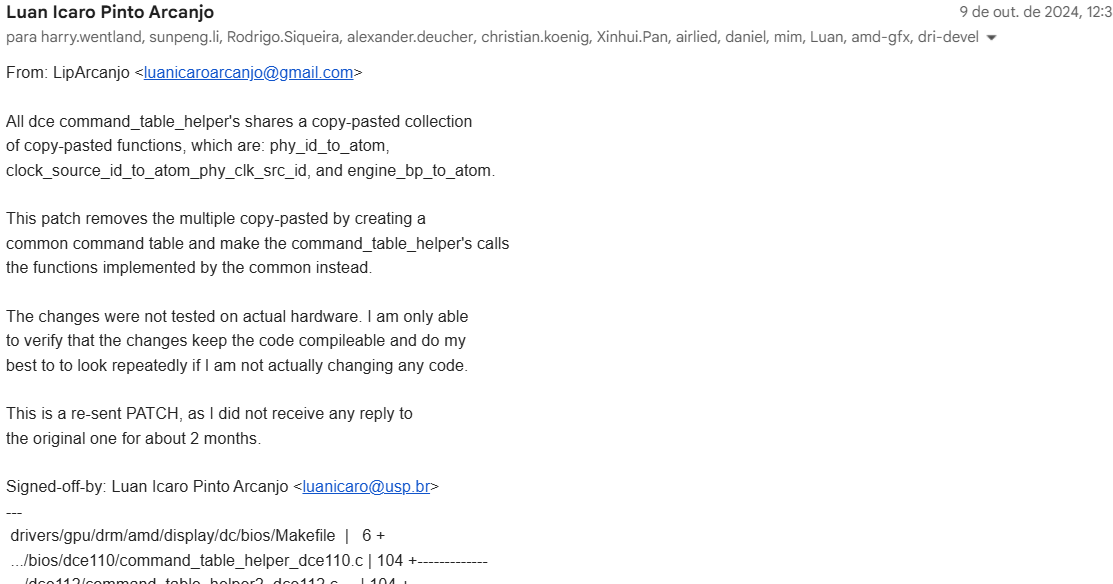
\includegraphics[scale=0.63]{patch_header}
\caption{List of issues in ArKanjo proposed to students to contribute}
\label{fig:issue_list}
\end{figure}

\newpage

\section{Students Contribution Reference}

Group 1 contribution was made through two change request.
The first change request can be accessed in the url: 
\url{https://github.com/LipArcanjo/arkanjo/pull/8}. 
The second change request can be accessed in the url: 
\url{https://github.com/LipArcanjo/arkanjo/pull/8}.

Group 2 contribution was splited in three change requests. The first change request
can be accessed in the url: \url{https://github.com/LipArcanjo/arkanjo/pull/7}.
The second change request can be accessed in the url:
\url{https://github.com/LipArcanjo/arkanjo/pull/9}. 
The third change request can be accessed in the 
url: \url{https://github.com/LipArcanjo/arkanjo/pull/11}.

\section{Documentation Webpage}

\begin{figure}
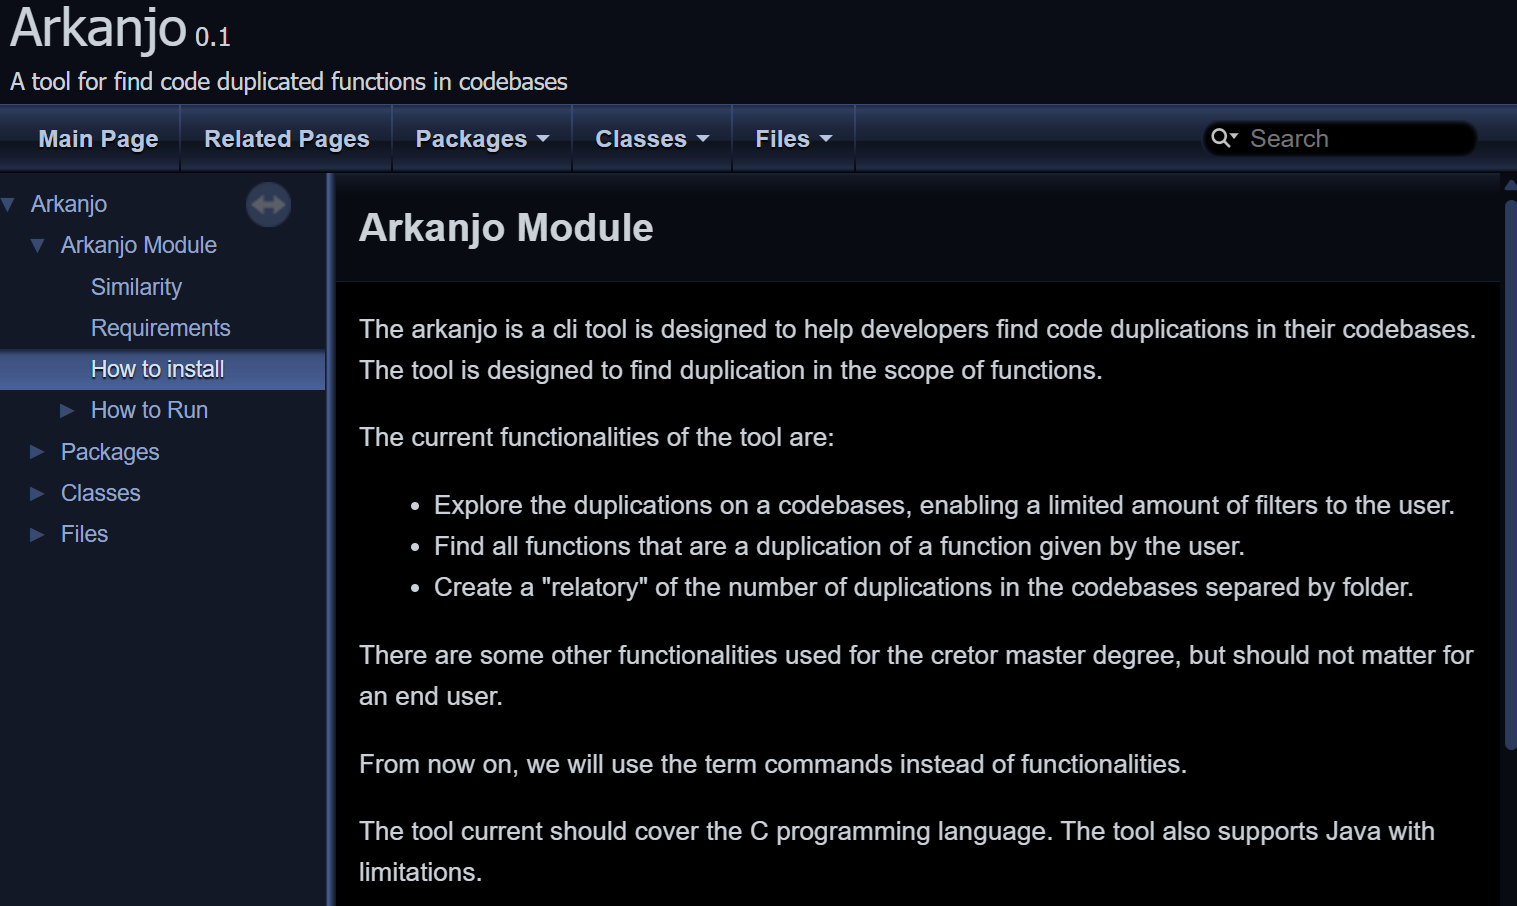
\includegraphics[scale=0.45]{webpage_1}
\caption{Documentation webpage - Main Page}
\label{fig:webpage1}
\end{figure}

\begin{figure}
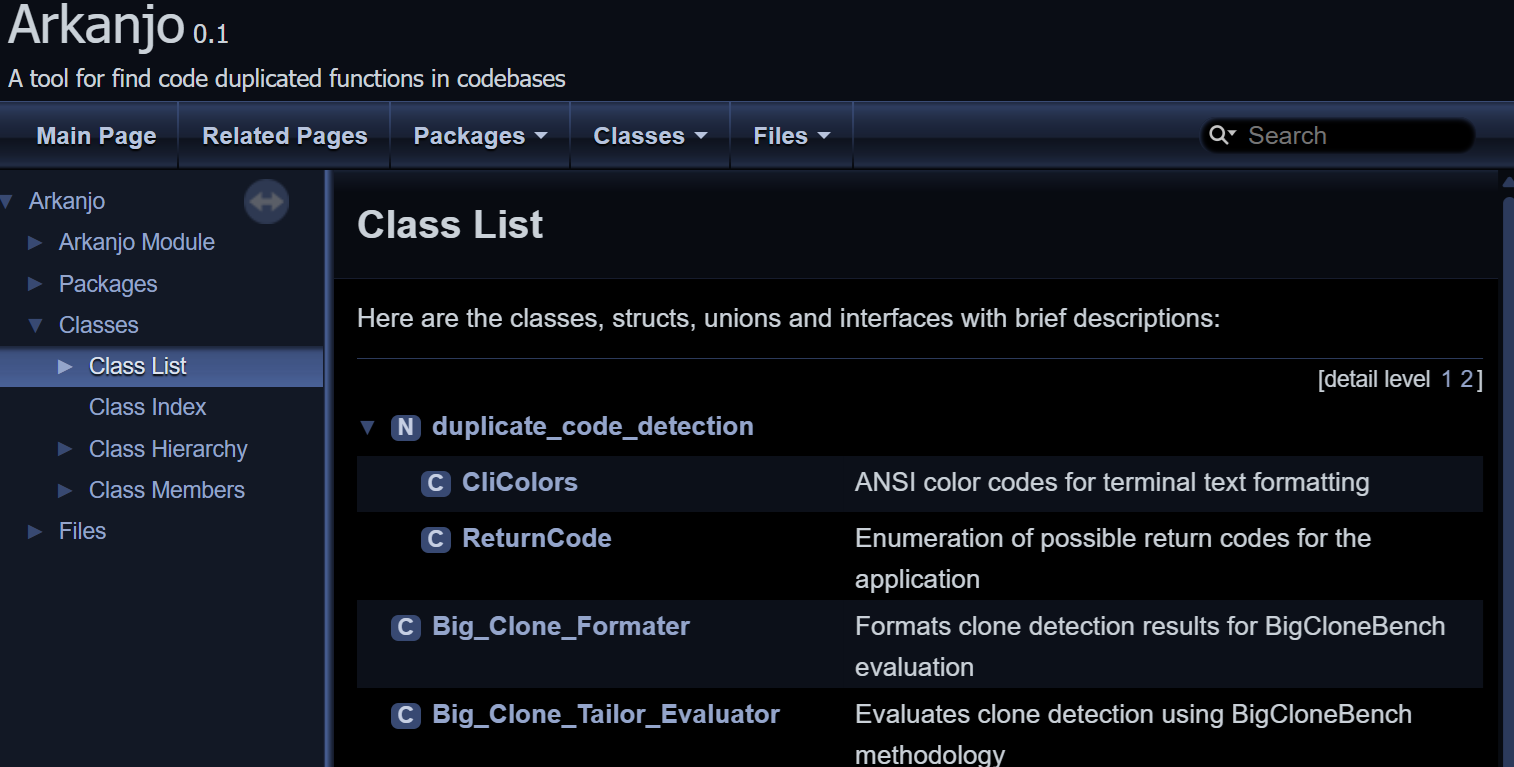
\includegraphics[scale=0.45]{webpage_2}
\caption{Documentation webpage - Class List Page}
\label{fig:webpage2}
\end{figure}
